\documentclass[tikz,border=8pt]{standalone}
\usepackage[T1]{fontenc}
\usepackage{lmodern}
\definecolor{rule}{HTML}{285D85}
\definecolor{current}{HTML}{548C7B}
\definecolor{history}{HTML}{B58A37}
\definecolor{collab}{HTML}{8B6C9E}
\begin{document}
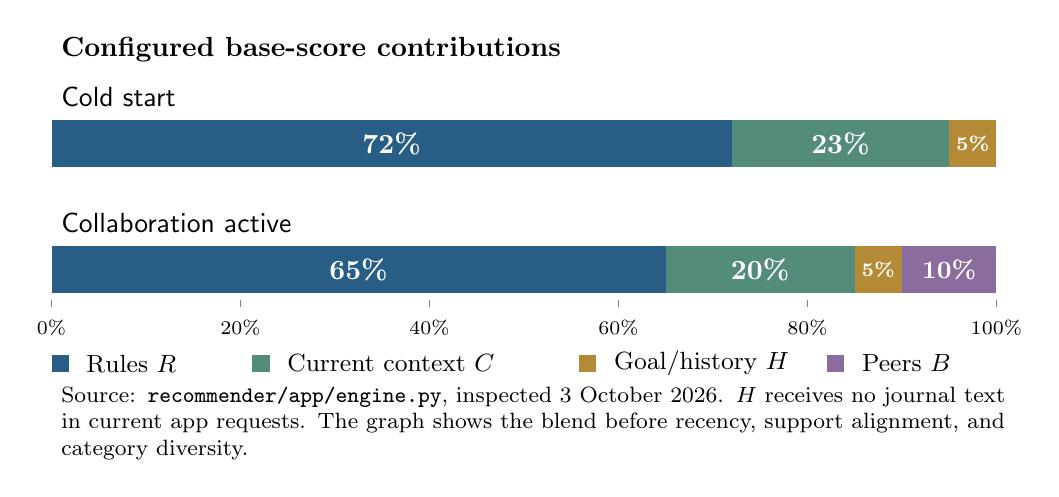
\begin{tikzpicture}[font=\sffamily]
\node[anchor=west,font=\bfseries] at (0,3.1) {Configured base-score contributions};
\node[anchor=west] at (0,2.5) {Cold start};
\node[anchor=west] at (0,0.9) {Collaboration active};
\fill[rule] (0,1.6) rectangle (8.64,2.2);
\fill[current] (8.64,1.6) rectangle (11.40,2.2);
\fill[history] (11.40,1.6) rectangle (12,2.2);
\node[text=white,font=\bfseries] at (4.32,1.9) {72\%};
\node[text=white,font=\bfseries] at (10.02,1.9) {23\%};
\node[text=white,font=\scriptsize\bfseries] at (11.7,1.9) {5\%};
\fill[rule] (0,0) rectangle (7.8,0.6);
\fill[current] (7.8,0) rectangle (10.2,0.6);
\fill[history] (10.2,0) rectangle (10.8,0.6);
\fill[collab] (10.8,0) rectangle (12,0.6);
\node[text=white,font=\bfseries] at (3.9,0.3) {65\%};
\node[text=white,font=\bfseries] at (9,0.3) {20\%};
\node[text=white,font=\scriptsize\bfseries] at (10.5,0.3) {5\%};
\node[text=white,font=\small\bfseries] at (11.4,0.3) {10\%};
\foreach \x/\n in {0/0,2.4/20,4.8/40,7.2/60,9.6/80,12/100} {
 \draw[gray] (\x,-0.08)--(\x,-0.17);
 \node[font=\scriptsize,anchor=north] at (\x,-0.22) {\n\%};
}
\fill[rule] (0,-1) rectangle (0.22,-0.78); \node[anchor=west,font=\small] at (0.32,-0.89) {Rules $R$};
\fill[current] (2.55,-1) rectangle (2.77,-0.78); \node[anchor=west,font=\small] at (2.87,-0.89) {Current context $C$};
\fill[history] (6.7,-1) rectangle (6.92,-0.78); \node[anchor=west,font=\small] at (7.02,-0.89) {Goal/history $H$};
\fill[collab] (9.85,-1) rectangle (10.07,-0.78); \node[anchor=west,font=\small] at (10.17,-0.89) {Peers $B$};
\node[anchor=west,text width=12cm,font=\footnotesize] at (0,-1.65) {Source: \texttt{recommender/app/engine.py}, inspected 3 October 2026. $H$ receives no journal text in current app requests. The graph shows the blend before recency, support alignment, and category diversity.};
\end{tikzpicture}
\end{document}
